%\iffalse (meta-comment)
%%  Copyright (C) 2010 by GuIT - Gruppo Utilizzatori Italiani di TeX
%%			<guit(at)sssup.it>
%%
%% This file may be distributed and/or modified under the conditions of
%% the LaTeX Project Public License, either version 1.2 of this license
%% or (at your option) any later version.  The latest version of this
%% license is in:
%% 
%%    http://www.latex-project.org/lppl.txt
%% 
%% and version 1.2 or later is part of all distributions of LaTeX version
%% 1999/12/01 or later.
%\fi
%
%\iffalse
%<driver>\ProvidesFile{guitbeamer.dtx}
%<class>\NeedTeXFormat{LaTeX2e}
%<class>\ProvidesClass{guitbeamer}
%<class>    [2010/03/03 v0.5 GuIT modified Beamer]
%<*driver>
\documentclass{ltxdoc}
\usepackage[color]{guit}

\newcommand{\email}[1]{\texttt{#1}}
\newcommand{\lcap}{{\fontencoding{T1}\selectfont\guillemotleft}}
\newcommand{\rcap}{{\fontencoding{T1}\selectfont\guillemotright}}
\newcommand{\Cap}[1]{\lcap #1\rcap}

\newcommand{\pkg}[1]{\textsf{#1}}
\let\cls\pkg
\newcommand{\env}[1]{\texttt{#1}}
%\iffalse
% \newcommand{\cmd}[1]{\texttt{\bs #1}}
%\fi
\newcommand{\cmdarg}[2]{\texttt{\bs #1\lb #2\rb}}

\EnableCrossrefs
% \DisableCrossrefs
\RecordChanges
\OnlyDescription
\CheckSum{0}

\begin{document}
\DocInput{guitbeamer.dtx}
\end{document}
%</driver>
%\fi
% \GetFileInfo{guitbeamer.dtx}
% %\DoNotIndex{}
%
% \title{La classe per presentazioni \pkg{guitbeamer}}
% \author{{\LARGE\GuIT} --- \GuITtext\thanks{\cls{guitbeamer} \`e stata
% scritta da Emiliano Giovanni Vavassori
% (\email{testina@sssup.it}). Si veda
% la sezione \ref{sec:acknow}.}}
% \date{Versione 0.5 --- 29 agosto 2006}
%  
% \maketitle
% 
% \begin{abstract}
% Viene qui presentata l'interfaccia dei comandi della classe
% \cls{guitbeamer}, scritta appositamente per rendere più semplice la
% produzione di diapositive per lezioni di \LaTeX. La classe si basa
% sulla ben più conosciuta classe \cls{beamer}.
% \end{abstract}
% 
% \tableofcontents
% \newpage
% \section*{Note di \textit{copyright}}
% La classe \cls{guitbeamer} è rilasciata sotto licenza
% $\!$\cc$\!\!\!$ Creative Commons 2.5\footnote{Il testo completo
% della licenza è disponibile, in inglese, alla pagina
% \url{http://creativecommons.org/licenses/by-nc-sa/2.5/legalcode}.}.
% 
% \noindent\emph{Tu sei libero di:}
% \begin{dinglist}{227}
%     \item di riprodurre, distribuire, comunicare al pubblico, esporre
% 	in pubblico, rappresentare, eseguire e recitare quest'opera;
%     \item di modificare quest'opera.
% \end{dinglist}
% 
% \noindent\emph{Alle seguenti condizioni:}
% \begin{description}
%     \item[\ccby Attribuzione]Devi attribuire la paternità dell'opera
% 	nei modi indicati dall'autore o da chi ti ha dato l'opera in
% 	licenza.
%     \item[\ccnc Non commerciale]Non puoi usare
% 	quest'opera per fini commerciali.
%     \item[\ \ccsa\ \ $\!\!$Condividi allo stesso modo]Se alteri o
% 	trasformi quest'opera, o se la usi per crearne un'altra, puoi
% 	distribuire l'opera risultante solo con una licenza identica a
% 	questa.
% \end{description}
% 
% \begin{dinglist}{52}
%     \item Ogni volta che usi o distribuisci quest'opera, devi farlo
% 	secondo i termini di questa licenza, che va comunicata con
% 	chiarezza.
%     \item In ogni caso, puoi concordare col titolare dei diritti
% 	d'autore utilizzi di quest'opera non consentiti da questa
% 	licenza.
% \end{dinglist}
% 
% Vorremmo mettere in particolare risalto il fatto che l'uso standard di
% questa classe (produzione di \textit{slides}) non è soggetto ai
% termini dell'opzione \emph{Condividi allo stesso modo}: pertanto, è
% possibile omettere l'indicazione della licenza sulle proprie
% \textit{slides}, ma è opportuno indicare, nei sorgenti, che
% \cls{guitbeamer} è soggetta alla licenza CCPL:
% \begin{verbatim}
% % guitbeamer.cls is under CCPL 2.5 - please see class file
% \documentclass[...]{guitbeamer}
% \end{verbatim}
% 
% \section{Introduzione}
% L'utilizzo delle diapositive (o, in inglese, \textit{slides}) in
% ambiente didattico risulta essere uno strumento fondamentale per
% catturare l'attenzione del discente; tale attenzione viene infatti
% aumentata con l'utilizzo di particolari effetti grafici e/o colori.
% 
% \`E tuttavia necessario far attenzione a non abusare di questi
% espedienti grafici per evitare di ottenere l'effetto diametralmente
% opposto: tipicamente, l'attenzione dell'auditorio verrebbe
% completamente assorbita dagli effetti grafici e sviata dall'oggetto
% della presentazione su qualcosa di molto più frivolo.
% 
% Questo è un rischio che può correre anche il docente che \Cap{perde
% energie} per sviluppare una presentazione visivamente molto efficace
% ma con contenuti di qualità sicuramente inferiore.
% 
% \cls{beamer} viene incontro alle persone che si trovano a dover
% presentare, spiegare, approfondire un argomento, permettendo loro di
% evitare questi problemi e focalizzando l'attenzione sui contenuti
% della presentazione, in pieno accordo con la filosofia di \LaTeX.
% 
% La classe \cls{guitbeamer} aggiunge alla potenza di \cls{beamer} una
% interfaccia di comandi semplificata e ottimizzata per la presentazione
% di argomenti correlati a \LaTeX, oltre che una serie di impostazioni
% grafiche studiate \emph{ad hoc}. Per ottenere tale risultato, sono
% stati posti i seguenti obiettivi: 
% \begin{itemize}
%   \item Razionalizzare i sorgenti delle \emph{slides}, così da evitare
%     che l'occhio di chi presenta si perda nel codice piuttosto che sul
%     contenuto;
%   \item Omogeneizzare il \textit{layout} delle singole \emph{slide}
%     all'interno di una stessa presentazione, per evitare, ad esempio,
%     che una classe venga \Cap{nominata} una volta con un carattere
%     \textit{sans-serif} e una volta con carattere \textit{typewriter}.
% \end{itemize}
% 
% La classe \cls{guitbeamer} è stata utilizzata successivamente per le 
% \Cap{Lezioni di \LaTeX} del \GuIT\ \cite{lez-latex05}.
% 
% \section{Compatibilità e apparenza}
% \cls{guitbeamer} non è un lavoro a se stante (ovviamente), ma è stata
% realizzata come \textit{collage} di stili predefiniti e di pacchetti
% caricati. Indichiamo in questa sezione le dipendenze della classe da
% eventuali altri pacchetti.
% 
% \subsection{Pacchetti caricati}
% La classe \cls{guitbeamer} carica automaticamente la classe
% \cls{beamer} per le presentazioni e restituisce un errore se essa non
% è per lo meno alla versione 3.05 (data di rilascio: 12/06/2005); il
% codice utilizzato nella classe è specifico ed utilizza istruzioni che
% sono rese disponibili solamente a partire da quella versione.
% 
% Gli altri pacchetti caricati, le opzioni specifiche utilizzate e
% l'eventuale richiesta di un numero di versione specifico sono tutte
% indicate in tabella~\ref{pacchetti}.
% \begin{table}[b]\centering
%   \caption{Pacchetti caricati nella classe \cls{guitbeamer}, relative
%   versioni richieste e opzioni utilizzate.}\label{pacchetti}
%   \medskip
%   \begin{tabular}{l c l}
%     \toprule
%     \emph{Nome pacchetto} & \emph{Vers. (Data di rilascio)} &
%     \emph{Opzioni utilizzate}\\
%     \midrule
%     \texttt{xcolor} & & \texttt{svgnames}\\
%     \texttt{graphicx} & &\\
%     \texttt{hyperref} & & \texttt{colorlinks=false}\\
%     \texttt{guit} & $\ge\,0.9$ (24/05/2006)& \texttt{color}\\
%     \bottomrule
%   \end{tabular}
% \end{table}
% Va da sé che le dipendenze dei pacchetti utilizzati devono essere, a
% loro volta, contemplate ed esaudite.
% 
% \subsection{Layout e grafica della presentazione}
% La classe utilizza il tema \Cap{Warsaw}, ne modifica il colore di
% struttura con quello ufficiale di \GuIT, carica l'\textit{outertheme}
% \Cap{split}, ridefinisce la \textit{footline}, imposta automaticamente
% l'istituzione di riferimento e, infine, carica i font serif solamente
% per la matematica. Se vi è sfuggito qualcosa di quanto appena esposto,
% vi consigliamo di dare una sbirciatina al manuale di \cls{beamer}
% \cite{manbeamer} oppure, a vostra discrezione, utilizzare la
% classe e guardarne l'output \texttt{:)}
% 
% \section{Interfaccia utente}
% All'interno della didattica legata a \LaTeX, il docente deve
% relazionare al pubblico non solo dell'utilizzo di un programma, ma
% anche alcune nozioni fondamentali all'intero della filosofia propria
% di \LaTeX; sono state studiate pertanto alcune macro per facilitare
% questo compito al relatore, fornendo un \textit{feedback} visuale alla
% spiegazione orale del docente.
% 
% Di seguito verranno descritti i comandi che sono introdotti dalla
% classe e come è possibile utilizzarli.
% 
% \subsection{Scrivere pacchetti, classi, ambienti}
% La classe rende disponibile alcuni comandi per evidenziare concetti
% particolari all'interno di \LaTeX:
% \begin{description}
% 	\item[\cmd{Lopt}]serve per evidenziare le opzioni che
% 		possono essere specificate ad una classe;
% 	\item[\cmd{Lsty}]è necessario per scrivere il nome di
% 	  pacchetti;
% 	\item[\cmd{Lcls}]evidenzia invece il nome delle classi;
% 	\item[\cmd{Lenv}]scrive il nome dell'ambiente che è
% 		necessario citare.
% \end{description}
% Essi richiedono tutti un argomento obbligatorio, che rappresenta per
% l'appunto il nome dell'oggetto particolare da nominare.
% 
% \subsection{Evidenziare}
% Una nota importante, prima di specificare i cambiamenti
% all'evidenziazione attuati nella classe. Esistono molti modi per
% evidenziare una parte di testo: fra tutti i modi che si possono
% scegliere, cambiare il colore del testo è quello, a nostro avviso, più
% \Cap{distruttivo} e fastidioso, anche se è al contempo quello più
% efficace. In \cls{guitbeamer} si fa già ricorso a parecchi colori,
% quindi valutate caso per caso se non convenga evidenziare con
% \verb+\emph+ oppure con \verb+\textbf+. Si ritiene preferibile
% utilizzare il grassetto nelle presentazioni che mutare il colore del
% testo, principalmente per due motivazioni:
% \begin{itemize}
%   \item il principale motivo per cui non si usa normalmente il
%     grassetto all'interno di un normale documento è perché \Cap{rompe
%     il colore del corpo del testo}. Tipicamente in una presentazione
%     si tende, per motivi di concisione, a scrivere brevi frasi e
%     pertanto non esiste un vero e proprio corpo del testo, inteso con
%     i canoni applicati ai documenti normali; è pertanto possibile e
%     non deleterio utilizzare il grassetto;
%   \item il grassetto è spesso utilizzato nel Web, che risulta essere
%     una delle applicazioni che più si avvicinano ad una presentazione
%     elettronica.
% \end{itemize}
% 
% Passando dalla teoria alla pratica, il comando \cmd{alert} di
% \cls{beamer} è stato ridefinito perché sia di colore blu; esso è stato
% preferito al colore rosso perché meno appariscente ma altrettanto
% d'effetto. Se necessario, è possibile ricorrere al nuovo comando
% \cmd{aalert} che invece evidenzia il suo argomento in rosso,
% esattamente come fa \verb+\alert+ di \cls{beamer}.
% 
% \subsection{Caratteri speciali}\label{sec:sp_char}
% Alcuni comandi della classe richiedono che qualche carattere speciale
% sia scritto in maniera un po' particolare: è il caso di
% tutti i comandi che seguiranno. In essi, sarà possibile (e in alcuni
% casi, necessario) indicare i caratteri speciali di \LaTeX\
% \texttt{\bs}, \texttt{\lb} e \texttt{\rb} come \verb+\\+, \verb+\{+ e
% \verb+\}+. L'eccezione è rappresentata da \verb+[+ e \verb+]+, che
% possono essere lasciate indicate normalmente o, nel caso non
% funzionino, sostituite dai meno diretti \verb+\ls+,
% \textit{left square (parenthesis)} e \verb+\rs+, \textit{right square
% (parenthesis)}. \`E stata scelta questa soluzione sia per ovviare ad un
% piccolo problema di natura estetica, sia perché necessario per alcuni
% comandi.
% 
% \subsection{Comandi per gli esempi}
% \subsubsection{Mostrare codice \LaTeX}
% Parlando di \LaTeX\ a qualunque livello, si finirà inevitabilmente,
% prima o poi, con il parlare di codice sorgente. \cls{guitbeamer}
% prevede un ambiente appositamente studiato per mostrare codice,
% \env{LaTeXcode}; esso è derivato da \env{semiverbatim} di \cls{beamer}
% e si consiglia pertanto di rileggere la documentazione di questo
% ambiente \cite{manbeamer} per capirne l'esatto funzionamento.
% 
% In questo ambiente è \emph{necessario} utilizzare quei simboli
% speciali definiti in \S~\ref{sec:sp_char}, quando si voglia
% \Cap{mostrare} tali caratteri speciali.
% 
% Altri comandi sono disponibili solo ed esclusivamente all'interno di
% questo ambiente:
% \begin{description}
% 	\item[\cmd{n}]Che rappresenta una singola interruzione di
% 	  riga (\emph{a capo});
% 	\item[\cmd{nn}]Che rappresenta una interruzione di riga
% 		doppia (quindi, una riga vuota);
% 	\item[\cmd{alert}]Per evidenziare parte del contenuto.
% 	  Necessita di un argomento obbligatorio, costituito dal testo
% 	  da evidenziare.
% \end{description}
% 
% \`E inoltre possibile specificare un titolo e un \textit{overlay} per
% l'ambiente \env{LaTeXcode} nello stesso modo in cui si fa con
% \cls{beamer}. Si veda, a tale scopo, il seguente esempio:
% \begin{Verbatim}[gobble=0]
% \begin{LaTeXcode}[Titolo del blocco]<3->
% 	ci metto un po' quello che voglio\\dots\n
% 	e \alert{apparir\\`a} correttamente\nn
% 	ciao a tutti
% \end{LaTeXcode}
% \end{Verbatim}
%  
% \subsubsection{Mostrare l'output di \LaTeX}
% Dopo aver spiegato il codice, è d'uopo mostrare il suo risultato:
%  anche per questo fine è stato predisposto un ambiente,
% \env{LaTeXoutput}. In questo caso, la sintassi è quella normale di
% \LaTeX\ e non è richiesta nessuna particolare sintassi nella
% composizione della parte, se si fa eccezione per:
% \begin{description}
%   \item[\cmd{noindent}]toglie il rientro (che è stato impostato di
%     \textit{default} dalla classe);
%   \item[\cmd{fakeind}]serve per inserire una falsa indentazione e va
%     usato a mano solo nei casi in cui non si ottiene l'indentazione
%     necessaria.
% \end{description}
% 
% Come il suo gemello per il codice, può anch'esso essere fornito di
% titolo e di specificazioni di \emph{overlay}, come mostrato
% nell'esempio:
% \begin{Verbatim}
% \begin{LaTeXoutput}[Titolo del blocco (output)]<4->
%   ci metto un po' quello che voglio\dots e apparir\`a correttamente
%   
%   ciao a tutti
% \end{LaTeXoutput}
% \end{Verbatim}
% 
% \subsubsection{Comandi \LaTeX\ nel corpo del testo}
% Sono state definite due macro, \cmd{LCmd} e \cmd{LCmdArg}, che
% permettono di evidenziare il codice all'interno del testo. Queste due
% macro sono comode quando si voglia, ad esempio, citare un comando
% (\verb+\listfiles+) e si voglia evidenziare l'argomento di un comando
% (\verb+\vspace{5em}+), rispettivamente.
% 
% La sintassi di \cmd{LCmd} prevede un argomento opzionale e uno
% obbligatorio. L'argomento opzionale (e quindi racchiuso fra le
% parentesi quadre \verb+[ ]+) è il carattere di \emph{inizio comando} o
% \textit{escape}, che di \textit{default} è settato a \verb+\+.
% L'argomento obbligatorio risulta invece essere il nome del comando che
% si vuole mostrare. Il comando \verb+\LCmd+ può inoltre essere inserito
% in un titolo di \textit{slide}: in tal caso perde il suo colore
% normale (blu scuro).
% 
% Facendo alcuni esempi, possiamo dire che \verb+\LCmd[]{pippo}+
% produce, nell'output, qualcosa di simile a \texttt{pippo}. \`E
% possibile, inoltre, scrivere un comando fornito di argomenti senza
% evidenziarli, utilizzando i caratteri speciali illustrati in
% \S~\ref{sec:sp_char} e potendo così scrivere
% \verb+\LCmd{documentclass[a4paper]\{article\}}+, che dà luogo a
% qualcosa di simile a \verb+\documentclass[a4paper]{article}+.
% 
% Il comando \verb+\LCmdArg+ invece non è utilizzabile nei titoli,
% prevede solamente due argomenti obbligatori ed è
% necessario per evidenziare l'argomento di un comando; ad esempio, per
% citare il caso precedente, si può utilizzare:\\[.5em]
% \verb+\LCmdArg{documentclass[a4paper]}{article}+\\[.5em] ed
% evidenziare così la classe del documento.
% 
% In entrambi i casi, ricordiamo nuovamente che possono essere
% utilizzati i caratteri di cui alla sezione \S~\ref{sec:sp_char}.
% 
% 
% \newpage
% \section{Esempi di \textit{slides}}
% In questa piccolissima sezione, analizzeremo alcune slides e il loro
% output, giusto per dare un'idea al lettore di come possano essere
% utilizzati i comandi della classe.
% 
% \subsection*{Esempio 1}\label{ex1}
% 
% \begin{Verbatim}[gobble=2]
%   \begin{frame}
%     \frametitle{Scrivere i loghi}
%     Ecco come si scrivono i loghi:
%     \begin{LaTeXcode}
%       \\TeX\n
%       \\LaTeX\n
%       \\LaTeXe
%     \end{LaTeXcode}
%     \medskip
%     \begin{LaTeXoutput}
%       \TeX\\
%       \LaTeX\\
%       \LaTeXe
%     \end{LaTeXoutput}
%   \end{frame}
% \end{Verbatim}
% 
% \bigskip
% \begin{center}
%   \fbox{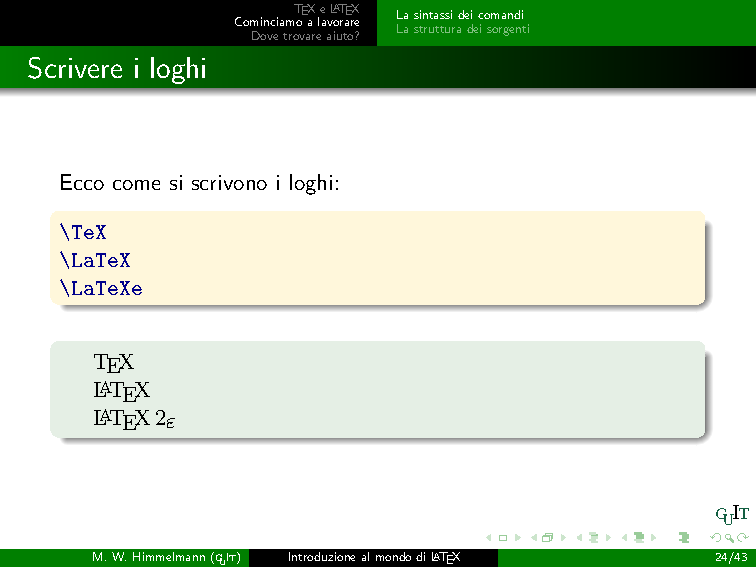
\includegraphics[width=.9\textwidth]{latexsymb}}
% \end{center}
% 
% \newpage 
% \subsection*{Esempio 2}\label{ex2}
% 
% \begin{Verbatim}[gobble=0]
% \begin{frame}
%   \frametitle{Il modello di un documento}
%   \begin{LaTeXcode}
%     \\documentclass[\alert{<opzioni>}]\{\alert{<classe>}\}\n
%     \onslide<2->
%     \quad\alert{<preambolo>}\nn
%     \onslide<3->
%     \\begin\{document\}\n
%     \onslide<4->
%     \alert{\quad<testo del documento>}\n
%     \onslide<3->
%     \\end\{document\}
%   \end{LaTeXcode}
% \end{frame}
% \end{Verbatim}
% 
% \bigskip
% \begin{center}
%   \fbox{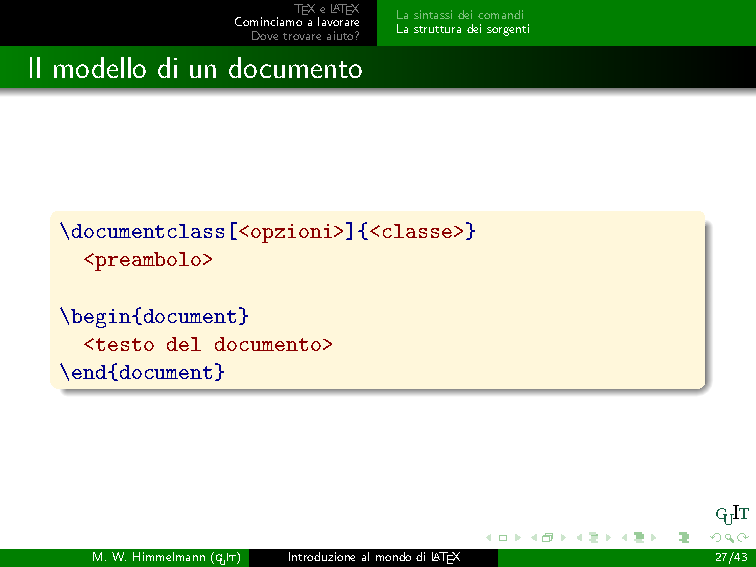
\includegraphics[width=.9\textwidth]{docexem}}
% \end{center}
% 
% \newpage 
% \subsection*{Esempio 3}\label{ex3}
% \begin{Verbatim}
% \begin{frame}
%   \frametitle{La sintassi di base}
%   \begin{itemize}[<+->]
%     \item tutti i comandi cominciano sempre con un
%       \LCmd\
%     \item spesso il comando è il nome inglese dell'azione
%     \item il comando ``termina'' con uno spazio bianco o con un
%       altro comando:
%     \begin{LaTeXcode}<4->
%       \\comando \alert{<testo>}\n
%       \\comando\\altrocomando
%     \end{LaTeXcode}
%   \end{itemize}
%   \smallskip
%   \begin{block}{Attenzione!}<5->
%     \begin{center}
%       \LaTeX\ è \textit{case sensitive}!\\[.5em]
%       bisogna pertanto stare attenti a distinguere tra\\[.3em]
%       \alert{\large MAIUSCOLO} e \alert{\large minuscolo}
%     \end{center}
%   \end{block}
% \end{frame}
% \end{Verbatim}
% 
% \bigskip
% \begin{center}
%   \fbox{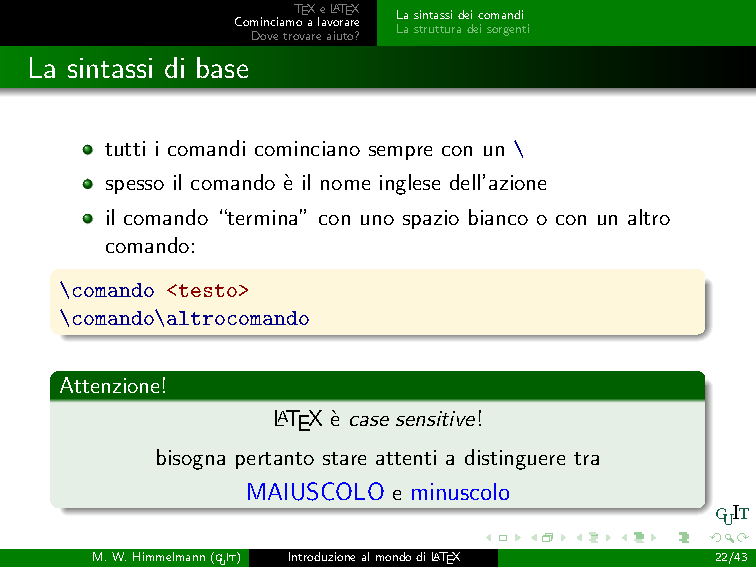
\includegraphics[width=.9\textwidth]{cmdexpl}}
% \end{center}
% 
% \newpage
% \subsection*{Esempio 4}\label{ex4}
% \begin{Verbatim}
% \begin{frame}
%   \frametitle{Due esempi di pacchetti}
%   \begin{LaTeXcode}
%     \\usepackage\{\alert{graphicx}\}
%   \end{LaTeXcode}
%   \Lsty{graphicx} è un pacchetto che permette di gestire l'inserimento
%   delle immagini, dei colori e di rotazioni
% 
%   \bigskip
%   \onslide<2->
%     \begin{LaTeXcode}
%       \\usepackage[\alert{italian}]\{\alert{babel}\}
%     \end{LaTeXcode}
%     \Lsty{babel} permette di sillabare testi scritti in lingue diverse 
%     dall'inglese (default), attivando la sillabazione della lingua
%     selezionata (in questo caso, la nostra: \LCmd[]{italian})
% \end{frame}
% \end{Verbatim}
% 
% \bigskip
% \begin{center}
%   \fbox{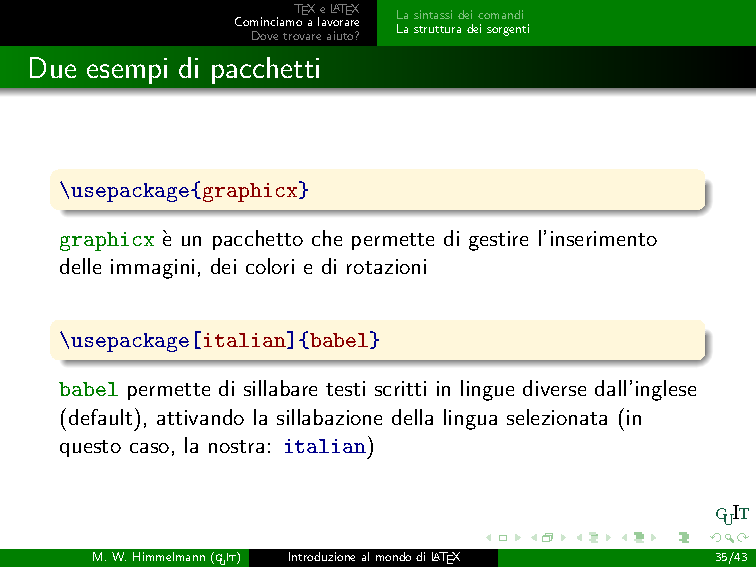
\includegraphics[width=.9\textwidth]{pkgexem}}
% \end{center}
% 
% \newpage
% \subsection*{Esempio 5}\label{ex5}
% \begin{Verbatim}
% \begin{frame}
%   \frametitle{Le classi base di \LaTeX}
%   \begin{LaTeXcode}
%     \\documentclass[<opzioni>]\{\alert{<classe>}\}
%   \end{LaTeXcode}
%   \begin{itemize}
%     \item\Lcls{article}
%     \item\Lcls{report}
%     \item\Lcls{book}
%     \item\Lcls{letter}
%     \item\Lcls{slides}
%     \item\dots
%     \item\Lcls{beamer}
%     \item\dots
%   \end{itemize}
% \end{frame}
% \end{Verbatim}
% 
% \bigskip
% \begin{center}
%   \fbox{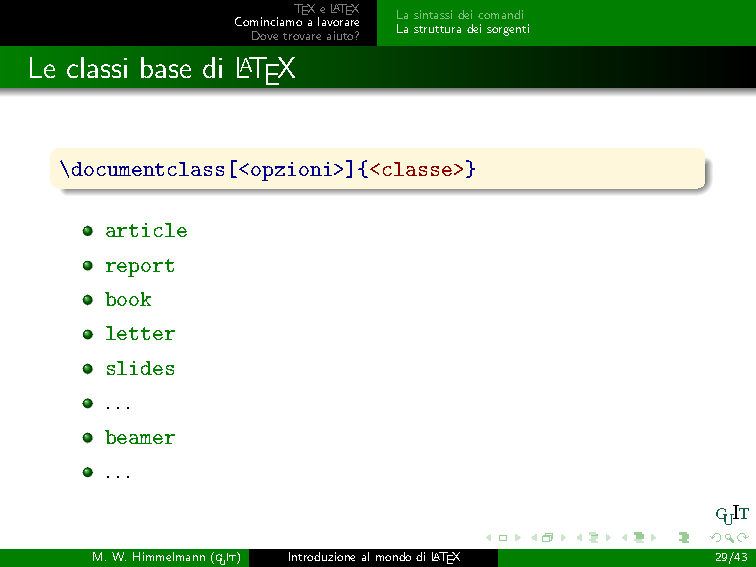
\includegraphics[width=.9\textwidth]{clsexpl}}
% \end{center}
% 
% \newpage
% \section{Ringraziamenti}\label{sec:acknow}
% Si ringraziano Maurizio Himmelmann e Fabiano Busdraghi che hanno fatto
% proposte e richieste precise in merito alla classe (alcune tutt'ora
% insolute, ad onor del vero) e sono stati veri e propri
% \textit{beta-testers} della classe.
% 
% Un sentito ringraziamento a Emanuele Vicentini, sempre prezioso e
% disponibile sia sul lato \TeX nico che su quello personale. Emanuele,
% ricorda che tutto ciò che hai dato ti sarà restituito 100 volte
% \texttt{:)}
% 
% \section{\textit{Disclaimer}, \textit{feedback} e \textit{bug
% reports}}\label{sec:fb&b}
% La presente classe non è stata scritta da un programmatore \LaTeX\
% professionista ed è pertanto da considerarsi soggetta a
% \textit{bugs}. Si invitano le persone che abbiano utilizzato questa
% classe a far pervenire all'autore, per mezzo della casella di posta
% elettronica \href{mailto:guit@sssup.it?subject=[guitbeamer]
% Feedback}{\texttt{guit@sssup.it}} eventuali richieste, commenti e
% segnalazioni di problemi su \cls{guitbeamer}, aggiungendo all'inizio
% del soggetto della mail la stringa ``\verb+[guitbeamer]+''.
% 
% \vfill
% \bibliographystyle{plain}
% \begin{thebibliography}{99}
%   \bibitem{lez-latex05} Maurizio W.~Himmelmann, Emiliano G.~Vavassori,
%     Fabiano Busdraghi; \newblock\emph{Introduzione al mondo di \LaTeX\ ---\
%     Guida al corso}, \newblock 2006, \GuITtext, Pisa.
%   \bibitem{manbeamer} Till Tantau; \newblock\emph{The \cls{beamer}
%     class}, manuale della classe, \newblock 2005.
% \end{thebibliography}
% \StopEventually{
%   \PrintChanges
%   \PrintIndex
% }
\RequirePackage[svgnames]{xcolor}
\LoadClassWithOptions{beamer}[2005/06/12]
\RequirePackageWithOptions{graphicx}
\hypersetup{colorlinks=false}

\RequirePackage[color]{guit}[2006/05/24]
\GuITcolor{1,.66,1,0}
% \iffalse (comment)
% Configurazioni di beamer
% \fi
\usetheme{Warsaw}
\beamertemplatenumberedballsectiontoc
\usecolortheme[rgb={0,.5,0}]{structure}
\useoutertheme{split}
\usefonttheme{default} 

% \iffalse (comment)
%%% Definisco il cmr per il testo matematico (come da pagina 174 della guida)
% \fi
\usetheme{Warsaw}
\usefonttheme[onlymath]{serif}

% \iffalse (comment)
%%% Colori dei blocchi di codice
% \fi
\usetheme{Warsaw}
\definecolor{LC background}{rgb}{1,.97,.86}
\colorlet{LC foreground}{DarkBlue}
\colorlet{LC alerted fg}{DarkRed}

\setbeamercolor{alerted text}{fg=blue}% Il colore degli alert e` blu
\setbeamercolor{aalerted text}{fg=red}% Il colore degli aalert e` rosso
\setbeamercolor{LaTeX code}{fg=LC foreground,bg=LC background}
\setbeamercolor{alerted LaTeX code}{fg=LC alerted fg,bg=LC background}

% \iffalse (comment)
%%% Ridefinisco la footline
% \fi
\setbeamertemplate{footline}{\leavevmode%
% \iffalse (comment)
% !! inserito hook per disattivare colorazione nella footline
% !! grazie a Gustavo Cevolani per la segnalazione
% \fi
\def\@inframetitle{pippo}%
\begin{beamercolorbox}[wd=.33\paperwidth,right,ht=2.25ex,dp=1ex,rightskip=4pt
  plus 1pt]{subsection in head/foot}
  \insertshortauthor\ (\insertshortinstitute)
\end{beamercolorbox}% 
\begin{beamercolorbox}[wd=.33\paperwidth,center,ht=2.25ex,dp=1ex]{section in head/foot}
  \usebeamercolor[fg]{section in foot/head}\insertshorttitle
\end{beamercolorbox}%
\begin{beamercolorbox}[wd=.34\paperwidth,ht=2.25ex,dp=1ex,leftskip=4pt plus 1pt,rightskip=4pt plus 1pt]{subsection in head/foot}
  \insertshortdate\hfill\insertframenumber/\inserttotalframenumber
\end{beamercolorbox}%
}

% \iffalse (comment)
%%% Ridefinisco il titolo per inserire un controllo
% \fi
\def\@inframetitle{}
\addtobeamertemplate{frametitle}{\def\@inframetitle{pippo}}

%
% \iffalse (comment)
% Definizioni utili
% \fi
%

% \iffalse (comment)
%%% Definisco un comando \aalert
%%% Utilizzo: \aalert{ argomento }
% \fi
\newcommand<>{\aalert}[1]{\begin{alertenv}#2\usebeamercolor[fg]{aalerted text}#1\end{alertenv}}

%
% \iffalse (comment)
% Comandi per la scrittura del codice LaTeX e del relativo output
% \fi
%
\newcommand{\bs}{{\char'134}}% Backslash
\newcommand{\lb}{{\char'173}}% Left brackets -> {
\newcommand{\rb}{{\char'175}}% Right brackets -> }
\newcommand{\ls}{{\char'133}}% Left brackets -> [
\newcommand{\rs}{{\char'135}}% Right brackets -> ]

%
% \iffalse (comment)
% Comandi per la scrittura di classi, pacchetti, ecc.
% \fi
%

% \iffalse (comment)
%%% Definisco il comando per nominare i pacchetti
%%% Utilizzo: \Lsty{ nome_classe_o_pacchetto }
%%% !! e' possibile utilizzarlo anche nei titoli
%%% !! Grazie a Gustavo Cevolani per la segnalazione
% \fi
\newcommand<>{\Lsty}[1]{%
\ifx\@inframetitle\@empty%
  \begin{actionenv}#2\usebeamercolor[fg]{structure}\ttfamily #1\end{actionenv}%
\else%
  \texttt{#1}%
\fi%
}
% \iffalse (comment)
%%% Definisco \Lcls nella stessa maniera di \Lsty
% \fi
\let\Lcls\Lsty
% \iffalse (comment)
%%% \Lopt e` un comando per nominare le opzioni delle classi
% \fi
\def\Lopt#1{\LCmd[]{#1}}
% \iffalse (comment)
%%% \Lenv e` un comando per nominare gli ambienti
% \fi
\let\Lenv\Lopt

% \iffalse (comment)
%%% LaTeXcode serve per scrivere codice in blocco a se stante ed
%%% e` basato sul codice di 'semiverbatim', classe beamer.
%%% Utilizzo: \begin{LaTeXcode}[ eventuale_titolo ]
%%%             \n \nn \alert{ }
%%%           \end{LaTeXcode}
% \fi
\newenvironment<>{LaTeXcode}[1][]%
{\begin{actionenv}#2%
  \def\insertblocktitle{#1}%
  \setbeamercolor{block body}{fg=LC foreground,bg=LC background}
  \newcommand{\n}{\newline}% Interruzione di riga singola
  \newcommand{\nn}{\newline\null\newline}% Interruzione di riga doppia
  \renewcommand*{\alert}[1]{{\usebeamercolor[fg]{alerted LaTeX code}##1}}% Alert
  \usebeamertemplate{block begin}\hbadness=10000%
  \begin{semiverbatim}}%
  {\end{semiverbatim}%
  \usebeamertemplate{block end}
\end{actionenv}}

% \iffalse (comment)
%%% LaTeXoutput serve per mostrare il risultato del codice.
%%% Utilizzo: \begin{LaTeXoutput}[ eventuale_titolo ]
%%%           \end{LaTeXoutput}
% \fi
\newenvironment<>{LaTeXoutput}[1][]%
{\begin{actionenv}#2%
  \def\insertblocktitle{#1}%
  \newcommand{\fakeind}{\hspace*{1.5em}}% Simula l'\indent. Va usato a mano
  \usebeamertemplate{block begin}\setlength{\parindent}{1.5em}\rmfamily}%
  {\usebeamertemplate{block end}
\end{actionenv}}

% \iffalse (comment)
%%% LCmd serve per scrivere un comando all'interno del testo.
%%% Utilizzo: \LCmd[ carattere_escape ]{ comando \\ \{ \} \ls \rs }
%%% NEW! Puo` essere usato anche nei titoli :)
% \fi
\newcommand{\LCmd}[2][\char'134 ]{\begingroup%
\let\\\bs\let\{\lb\let\}\rb%
\ifx\@inframetitle\@empty%
  \usebeamercolor[fg]{LaTeX code}\ttfamily{#1}{#2}%
\else%
  \ttfamily{#1}{#2}%
\fi%
\endgroup}

% \iffalse (comment)
%%% LCmdArg e` simile a LCmd ma mette in evidenza l'argomento.
%%% Utilizzo: \LCmdArg{ comando }{ argomento_del_comando }
%%% All'interno di \LCmdArg si possono usare gli stessi simboli di \LCmd.
% \fi
\newcommand{\LCmdArg}[2]{\begingroup%
\let\\\bs\let\{\lb\let\}\rb%
\color{LaTeX code.fg}\ttfamily\char'134{#1}\char'173{\color{alerted LaTeX code.fg}{#2}}\char'175\endgroup}

% \iffalse (comment)
%%% Per scrivere correttamente \, {, }, [ e ] nel testo
% \fi
\newcommand{\tbs}{\LCmd{}}% Textual BackSlash
\newcommand{\tlb}{\LCmd[]{\lb}}% Textual Left Bracket
\newcommand{\trb}{\LCmd[]{\rb}}% Textual Right Bracket
\newcommand{\tls}{\LCmd[]{\ls}}% Textual Left Square
\newcommand{\trs}{\LCmd[]{\rs}}% Textual Right Square

% \iffalse (comment)
%%% Impostiamo istituzione e logo
% \fi
\def\ncGuIT{\GuIT[color=no]}
\institute[\protect\ncGuIT]{\scalebox{2}{\GuIT} --- \large\GuITtext\\\GuITurl}
\logo{\scalebox{2}{\GuIT}}

% \Finale
\endinput
